\section{Propuesta}
Para garantizarle al usuario que la aplicación que implementa respeta
determinadas políticas de seguridad, el desarrollador Android requiere de una
herramienta que le permita: primero definir las políticas de seguridad a
evaluar, y segundo, verificar el cumplimiento de las políticas
definidas.\newline 
La propuesta para cumplir con tales requerimientos consiste en proveer una
herramienta de análisis de flujo de información, mediante el sistema de
anotaciones de Jif. Se parte de Jif porque ofrece un sistema de anotaciones
basado en un modelo de etiquetas(DLM), más un módulo de verificación(compilador
de Jif), tal como se ilustra en la figura \ref{fig:desingReal}. 
Así, mediante las etiquetas del DLM el desarrollador puede definir políticas de
seguridad en el código de su aplicación, para luego validar con el módulo de
verificación, si la aplicación respeta tales políticas.\newline 
Ahora bien, el diseño ideal para contribuir con la solución del problema es: una
herramienta que contenga el setup de Jif para Android, e integre un clasificador de sources
y sinks. De modo que, la herramienta analice flujos de información en
aplicativos Android, verificando que cumplan con las políticas de seguridad que
el desarrollador ha definido.\newline 
El Setup de Jif para Android consiste en las clases de la API Android con
anotaciones Jif(Anotaciones a la API), estas
anotaciones son necesarias porque la API permite que la aplicación escriba o lea
información de los sources y los sinks, generando flujos de información entre
estos. En consecuencia, para analizar el flujo de información entre sources y
sinks se requiere anotar las clases de la API.\newline
No obstante, para efectos del presente trabajo se limita el Setup de Jif,
partiendo de una política de seguridad específica.
Por consiguiente, el diseño se centra en soportar un conjunto reducido de clases
de la API de Android, y en incluir un conjunto específico de sources y
sinks; de acuerdo a una política de seguridad establecida. Ese conjunto de
sources y sinks, se toma del listado de sources y sinks proveído por SuSi
\ref{sec:susi}.\newline
Adicionalmente, para aspectos de evaluación, se incluye el diseño de un anotador
que automatiza la anotación requerida por el desarrollador.
De modo que, acorde a la política de seguridad establecida, se genere la
versión anotada del aplicativo a analizar.\newline
La figura \ref{fig:desingReal} muestra el esquema del diseño, allí los componentes
principales son el \emph{generador de anotaciones} y la \emph{herramienta de
análisis estático}.\newline 
Para retornar la versión Jif del aplicativo, el \emph{generador de anotaciones}
parte del código fuente de la aplicación Android a analizar, la política de
seguridad a evaluar, y los sources y sinks requeridos para verificar tal
política.\newline 
Luego esa versión Jif del aplicativo se debe pasar como entrada a la herramienta
de análisis estático, la cual retorna el análisis de flujo de
información.\newline 
La \emph{herramienta de análisis estático}, está integrada
por el compilador de Jif(Módulo de verificación) y las anotaciones a la API de
Android.

\begin{figure}[t!]
	\begin{center} 
	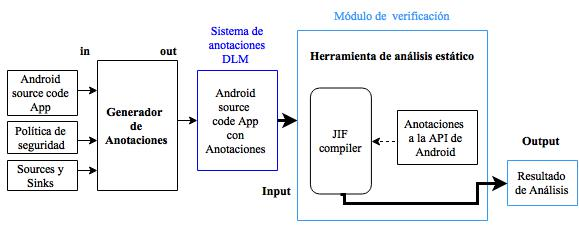
\includegraphics[width=8.8cm]{desing3Real-2-2-colors-2.jpg} 
	\end{center}
	\caption{Diseño herramienta de análisis estático.\newline
	Partiendo del código fuente del aplicativo Android, la política de seguridad a
	evaluar, más los sources y sinks requeridos para verificar la política; el
	generador de anotaciones retorna la versión anotada del aplicativo a analizar.
	Luego la versión anotada del aplicativo se pasa como entrada a la herramienta
	de análisis estático, la cual retorna el resultado de análisis de flujo de información.}
	\label{fig:desingReal}
\end{figure}

Siguiendo el esquema de diseño anteriormente descrito: primero, se define la
política de seguridad a evaluar \ref{subsection:politica}; segundo, se toman a
consideración elementos influyentes para verificar el cumplimiento de la
política mediante Jif \ref{subsec:consVerPol}; y tercero, teniendo en cuenta
\ref{subsection:politica} y \ref{subsec:consVerPol}, se definen los lineamientos
de anotación \ref{sec:lineamientos}. Tales lineamientos establecen el esquema
para anotaciones a la API Android y anotaciones a los aplicativos a
analizar(lineamientos del anotador).

\subsection{Definición de la política de seguridad}
% \textit{Definición de la política de seguridad}:
Detectar si una aplicación Android presenta flujos de información entre,
información con nivel de seguridad alto e información con nivel de seguridad bajo.\newline
\textit{Información considerada con nivel de seguridad alto}: la información
catalogada con nivel de seguridad alto hace referencia a un conjunto de sources.
Los sources representan información confidencial o privada del usuario, por
tanto, este quisiera tener el control de hacia donde se dirige tal información.
El conjunto de sources está integrado por los métodos getDeviceId,
getSimSerialNumber, findViewById, getLatitude, getLongitude y getSubscriberId.
Adicional a estos métodos, se incluye el tipo de dato EditText, si y sólo si, el
campo UI al que referencia corresponde a un campo tipo textPassword, campos
destinados a almacenar contraseñas.\newline 
\textit{Información considerada con nivel de seguridad bajo}: la
información considerada con nivel de seguridad bajo, comprende un conjunto
de sinks. Los sinks son canales que permiten la salida de información del
dispositivo, por ejemplo, los mensajes de texto. El conjunto de sinks
está integrado por los métodos de la clases Log y SmsManager de la API.\newline
Este conjunto de sources y sinks es tomado del listado proveído por el
clasificador SuSi \ref{sec:susi}.

\subsection{Lineamientos de anotación}
Los lineamientos de anotación definen los elementos básicos de anotación
\ref{subsec:elements}, anotaciones necesarias para la API de Android
\ref{subsec:api} y anotaciones en los aplicativos a analizar \ref{subsec:anotador}.

\subsubsection{Elementos básicos de anotación}
Para anotar la información con su respectivo nivel de seguridad alto o bajo, de
modo que, partiendo de tales anotaciones se evalúe la existencia de flujos de
información entre información con nivel de seguridad alto e información con
nivel de seguridad bajo, se define una autoridad para los programas, también se
definen los labels de seguridad para especificar las políticas de seguridad.
Así:\newline Principal \emph{Alice}: haciendo uso de los principals ya definidos en Jif, se
establece al principal \emph{Alice} como la autoridad máxima. Este principal
tendrá todo el poder para actuar sobre aspectos de los programas.\newline
Política para anotar información con nivel de seguridad alto: el label de
seguridad \emph{\{Alice:\}},  indica que la información tiene nivel seguridad
alto, es decir, que se trata de información sensible o privada.\\
Variables con nivel de seguridad alto deben ser anotadas con tal label de
seguridad, porque esté específica que sólo el dueño de la información(Alice)
puede acceder a la misma.\newline 
Política para anotar información con nivel de seguridad bajo: el label de
seguridad \emph{\{\}}, indica que la información tiene nivel de seguridad bajo,
es decir, información de conocimiento público.\newline


\subsubsection{Anotaciones a la API de Android}
\label{subsec:api}
%\textbf{(b)Anotaciones a la API de Android}\newline

\begin{figure}[t!]
	\begin{center}
	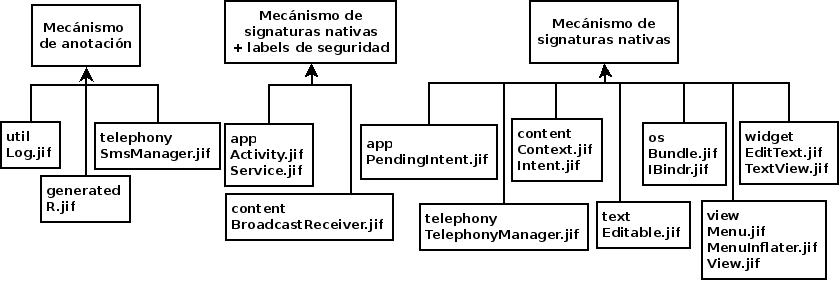
\includegraphics[width=8.5cm]{annotationsMechanims.jpeg}
	\end{center}
	\caption{Mecanismos de anotación para clases de la API.}
	\label{fig:annotationsMechanims}  
\end{figure}

Para controlar el flujo de información que se envía hacia sinks, la
definición de los métodos de las clases Log y SmsManager de la API Android,
deben anotarse de tal manera que, se controle el nivel de desde el
punto del programa donde es invocado el método, y el nivel de seguridad de los
argumentos con que se invocan tales métodos.\newline 
Para ello se recurre a los principios que regulan el llamado a métodos
en el sistema de anotaciones de Jif, entre los cuales está que, el nivel de
seguridad de los argumentos con que se invoca un método, debe ser menor o igual
de restrictivo que los labels de seguridad con que se ha definido
el método.
Tomando como ejemplo el método sendTextMessage de
la clase SmsManager, mediante el cual se envían mensajes de texto:
\begin{lstlisting}[basicstyle=\scriptsize]
sendTextMessage(String destinationAddress, String scAddress, 
String text, PendingIntent sentIntent, 
PendingIntent deliveryIntent)
\end{lstlisting}

Se tiene que el parámetro \emph{text} es el que recibe la información a mostrar,
y por tanto esa información debe ser pública.\newline 
Por consiguiente, en la definición del método el label de seguridad del
argumento(AL) correspondiente a la información a mostrar(logs) o la información
a enviar(sms), se anota con el label de seguridad bajo(label público\{\}). Con
esto se garantiza que la información se muestra o envía, si y sólo si, el nivel
de seguridad del argumento con que se invoca el método es público. Por ejemplo,
si el método se invoca con información anotada con label de seguridad alto, se
genera un flujo de información indebido, dando lugar a un error en la
compilación del programa que le llama.\newline 
El resto de argumentos del método se anotan con label de seguridad \{Alice:\},
puesto que esa información puede ser pública o privada.\newline
En el caso del BL al anotarlo con el label \{Alice:\}, se permite que el método
sea invocado desde cualquier punto de un programa. 
Para el resto de labels se dejan los que Jif genera por defecto.\newline
% cualquier punto de un programa que sea igual o menor de restrictivo que el
% principal Alice, esto se traduce en que podrá ser invocado desde cualquier punto
% de un programa, lo cual es correcto porque lo que se busca el evitar que se
% envíe información considerada con nivel se deguridad alto y no, evitar que el
% método sea utilizado. Poner ejemplo XXXX?\newlie
Continuando con el ejemplo del método sendTextMessage y aplicando lo
anteriormente descrito, este método se anota de la siguiente manera:
\begin{lstlisting}
sendTextMessage{Alice:}(String{Alice:} destinationAddress, 
	String{Alice:}scAddress, 
	String{} text, 
	PendingIntent{Alice:} sentIntent,
	PendingIntent{Alice:} deliveryIntent) { }
\end{lstlisting}





















